\hypertarget{a00336}{}\section{M\+I\+D\+I}
\label{a00336}\index{M\+I\+D\+I@{M\+I\+D\+I}}
How to route and process M\+I\+D\+I in A\+A\+X plug-\/ins. 

\hypertarget{a00336_additionalFeatures_MIDI_Overview}{}\subsection{Midi Overview}\label{a00336_additionalFeatures_MIDI_Overview}
Direct\+Midi is Avid\textquotesingle{}s protocol for communication of M\+I\+D\+I and other timing-\/critical plug-\/in information. It is a cross-\/platform solution to tightly integrate the host application, audio engine, and plug-\/ins.\hypertarget{a00336_additionalFeatures_MIDI_NodeTypes}{}\subsection{M\+I\+D\+I node types}\label{a00336_additionalFeatures_MIDI_NodeTypes}
There are four kinds of nodes an A\+A\+X plug-\/in can create. See \hyperlink{a00206_a5e1dffce35d05990dbbad651702678e4}{A\+A\+X\+\_\+\+E\+M\+I\+D\+I\+Node\+Type} for additional details about these node types\+: \begin{DoxyItemize}
\item \hyperlink{a00206_a5e1dffce35d05990dbbad651702678e4ae57de2b04978fe2e75f5bdeb034bda44}{A\+A\+X\+\_\+e\+M\+I\+D\+I\+Node\+Type\+\_\+\+Local\+Input} \item \hyperlink{a00206_a5e1dffce35d05990dbbad651702678e4acc1b5f2109c508b20a65b5e0fdcd643f}{A\+A\+X\+\_\+e\+M\+I\+D\+I\+Node\+Type\+\_\+\+Local\+Output} \item \hyperlink{a00206_a5e1dffce35d05990dbbad651702678e4a2be91828f8c1dac20ab5dff136fc1fce}{A\+A\+X\+\_\+e\+M\+I\+D\+I\+Node\+Type\+\_\+\+Global} \item \hyperlink{a00206_a5e1dffce35d05990dbbad651702678e4ac2ff856aec0724907dfd95b8e3ccbc20}{A\+A\+X\+\_\+e\+M\+I\+D\+I\+Node\+Type\+\_\+\+Transport}\end{DoxyItemize}
\hypertarget{a00336_additionalFeatures_MIDI_AddingMIDI}{}\subsection{Adding M\+I\+D\+I functionality to a plug-\/in}\label{a00336_additionalFeatures_MIDI_AddingMIDI}
Plug-\/in may access M\+I\+D\+I data in its algorithm or data model. If plug-\/in needs M\+I\+D\+I in both places or just in the algorithm, it should add a M\+I\+D\+I node to the algorithm context, i.\+e. call \hyperlink{a00088_a6284dda9ccca898e33075de29dad4e39}{A\+A\+X\+\_\+\+I\+Component\+Descriptor\+::\+Add\+M\+I\+D\+I\+Node()} with the appropriate node type.


\begin{DoxyCode}
\textcolor{comment}{//==============================================================================}
\textcolor{comment}{// Algorithm context definitions}
\textcolor{comment}{//==============================================================================}

\textcolor{comment}{// Context structure}
\textcolor{keyword}{struct }SMy\_Alg\_Context
\{
    [...]
    \hyperlink{a00105}{AAX\_IMIDINode}  * mMIDIInNodeP;         \textcolor{comment}{// Local input MIDI node pointer}
    \hyperlink{a00105}{AAX\_IMIDINode}  * mMIDINodeOutP;        \textcolor{comment}{// Local output MIDI node pointer}
    \hyperlink{a00105}{AAX\_IMIDINode}  * mMIDINodeTransportP;  \textcolor{comment}{// Transport node }
    [...]
\};

\textcolor{keyword}{enum} EDemoMIDI\_Alg\_PortID
\{
    [...]
    \textcolor{comment}{//}
    \textcolor{comment}{// Add the MIDI node as a physical address within the context field}
    ,eAlgPortID\_MIDINodeIn          = \hyperlink{a00149_acf807247ecd6e5899dc9dc31644e9a1d}{AAX\_FIELD\_INDEX} (SDemoMIDI\_Alg\_Context, mMIDINodeP)
    ,eAlgPortID\_MIDINodeOut         = \hyperlink{a00149_acf807247ecd6e5899dc9dc31644e9a1d}{AAX\_FIELD\_INDEX} (SDemoMIDI\_Alg\_Context, mMIDINodeOutP)
    ,eAlgPortID\_MIDINodeTransport   = \hyperlink{a00149_acf807247ecd6e5899dc9dc31644e9a1d}{AAX\_FIELD\_INDEX} (SDemoMIDI\_Alg\_Context, 
      mMIDINodeTransportP)
    [...]
\};
\end{DoxyCode}



\begin{DoxyCode}
\textcolor{comment}{// ***************************************************************************}
\textcolor{comment}{// ROUTINE: DescribeAlgorithmComponent}
\textcolor{comment}{// Algorithm component description}
\textcolor{comment}{// ***************************************************************************}
\textcolor{keyword}{static} \textcolor{keywordtype}{void} DescribeAlgorithmComponent( \hyperlink{a00088}{AAX\_IComponentDescriptor} * outDesc )
\{
    \hyperlink{a00149_a4d8f69a697df7f70c3a8e9b8ee130d2f}{AAX\_Result}                    err;
    
    [...]
    \textcolor{comment}{// Register MIDI nodes}
    err = outDesc->\hyperlink{a00088_a6284dda9ccca898e33075de29dad4e39}{AddMIDINode}(eAlgPortID\_MIDINodeA, 
      \hyperlink{a00206_a5e1dffce35d05990dbbad651702678e4ae57de2b04978fe2e75f5bdeb034bda44}{AAX\_eMIDINodeType\_LocalInput}, \textcolor{stringliteral}{"DemoMIDI"}, 0xffff);                  
      \hyperlink{a00158_a168ee44fd7a5485ab50160db36fb2988}{AAX\_ASSERT} (err == 0);
    err = outDesc->\hyperlink{a00088_a6284dda9ccca898e33075de29dad4e39}{AddMIDINode}(eAlgPortID\_MIDINodeOut, 
      \hyperlink{a00206_a5e1dffce35d05990dbbad651702678e4acc1b5f2109c508b20a65b5e0fdcd643f}{AAX\_eMIDINodeType\_LocalOutput}, \textcolor{stringliteral}{"DemoMIDIOut"}, 0xffff);         
      \hyperlink{a00158_a168ee44fd7a5485ab50160db36fb2988}{AAX\_ASSERT} (err == 0);
    err = outDesc->\hyperlink{a00088_a6284dda9ccca898e33075de29dad4e39}{AddMIDINode}(eAlgPortID\_MIDINodeTransport, 
      \hyperlink{a00206_a5e1dffce35d05990dbbad651702678e4ac2ff856aec0724907dfd95b8e3ccbc20}{AAX\_eMIDINodeType\_Transport}, \textcolor{stringliteral}{"DemoMIDITrnsprt"}, 0xffff); 
      \hyperlink{a00158_a168ee44fd7a5485ab50160db36fb2988}{AAX\_ASSERT} (err == 0);
    [...]
\}
\end{DoxyCode}


If M\+I\+D\+I data is needed in the plug-\/in\textquotesingle{}s data model only, plug-\/in should describe M\+I\+D\+I node with \hyperlink{a00096_aa7709de005e0256feb522758ccc5b582}{A\+A\+X\+\_\+\+I\+Effect\+Descriptor\+::\+Add\+Control\+M\+I\+D\+I\+Node()}.


\begin{DoxyCode}
\textcolor{comment}{// ***************************************************************************}
\textcolor{comment}{// ROUTINE: GetPlugInDescription}
\textcolor{comment}{// ***************************************************************************}
\textcolor{keyword}{static} \hyperlink{a00149_a4d8f69a697df7f70c3a8e9b8ee130d2f}{AAX\_Result} GetPlugInDescription( \hyperlink{a00096}{AAX\_IEffectDescriptor} * 
      outDescriptor )
\{
    \hyperlink{a00149_a4d8f69a697df7f70c3a8e9b8ee130d2f}{AAX\_Result}                    err;
    
    [...]
    \textcolor{comment}{// Register MIDI nodes}
    err = outDesc->AddControlMIDINode(\textcolor{stringliteral}{'linp'}, \hyperlink{a00206_a5e1dffce35d05990dbbad651702678e4ae57de2b04978fe2e75f5bdeb034bda44}{AAX\_eMIDINodeType\_LocalInput}, \textcolor{stringliteral}{"
      DemoMIDI"}, 0xffff);        \hyperlink{a00158_a168ee44fd7a5485ab50160db36fb2988}{AAX\_ASSERT} (err == 0);
    err = outDesc-> AddControlMIDINode(\textcolor{stringliteral}{'lout'}, \hyperlink{a00206_a5e1dffce35d05990dbbad651702678e4acc1b5f2109c508b20a65b5e0fdcd643f}{AAX\_eMIDINodeType\_LocalOutput}, \textcolor{stringliteral}{
      "DemoMIDIOut"}, 0xffff);  \hyperlink{a00158_a168ee44fd7a5485ab50160db36fb2988}{AAX\_ASSERT} (err == 0);
    err = outDesc-> AddControlMIDINode(\textcolor{stringliteral}{'tran'}, \hyperlink{a00206_a5e1dffce35d05990dbbad651702678e4ac2ff856aec0724907dfd95b8e3ccbc20}{AAX\_eMIDINodeType\_Transport}, \textcolor{stringliteral}{"
      DemoMIDITrnsprt"}, 0xffff);  \hyperlink{a00158_a168ee44fd7a5485ab50160db36fb2988}{AAX\_ASSERT} (err == 0);
    [...]

    \textcolor{keywordflow}{return} err;
\}
\end{DoxyCode}


\begin{DoxyNote}{Note}
These two types of M\+I\+D\+I nodes can\textquotesingle{}t be used together in the same plug-\/in\textquotesingle{}s effect.
\end{DoxyNote}
\hypertarget{a00336_additionalFeatures_MIDI_Algorithm}{}\subsection{Using M\+I\+D\+I in a plug-\/in algorithm}\label{a00336_additionalFeatures_MIDI_Algorithm}
Like with other algorithm context ports, data in M\+I\+D\+I nodes is directly available in the plug-\/in\textquotesingle{}s algorithm process function. Here is an example from the Demo\+M\+I\+D\+I\+\_\+\+Note\+On sample plug-\/in\+:


\begin{DoxyCode}
\textcolor{keyword}{template}<\textcolor{keywordtype}{int} kNumChannelsIn, \textcolor{keywordtype}{int} kNumChannelsOut> 
\textcolor{keywordtype}{void}
\hyperlink{a00149_aaa22112139aa627574b1ef562f579d43}{AAX\_CALLBACK}
DemoMIDI\_AlgorithmProcessFunction (
                                   SDemoMIDI\_Alg\_Context * \textcolor{keyword}{const}    inInstancesBegin [],
                                   \textcolor{keyword}{const} \textcolor{keywordtype}{void} *                 inInstancesEnd)
\{
    [...]
    \textcolor{comment}{// Setup MIDI In node pointers }
    \hyperlink{a00105}{AAX\_IMIDINode}* midiNodeIn = instance->mMIDINodeP;
    \hyperlink{a00025}{AAX\_CMidiStream}* midiBufferIn = midiNodeIn->\hyperlink{a00105_a794f1c0d19ac6720382c23b0a4dc2b17}{GetNodeBuffer}();
    \hyperlink{a00024}{AAX\_CMidiPacket}* midiBufferInPtr = midiBufferIn->\hyperlink{a00025_a5011ea886dce57b382c23b82e56d3000}{mBuffer};
    uint32\_t packets\_count\_in = midiBufferIn->\hyperlink{a00025_ad93c962a8278977f2a4f07b1e7490a90}{mBufferSize};
    
    \textcolor{comment}{// Setup MIDI Out node pointers }
    \hyperlink{a00105}{AAX\_IMIDINode}* midiNodeOut = instance->mMIDINodeOutP;
    \hyperlink{a00025}{AAX\_CMidiStream}* midiBufferOut = midiNodeOut->\hyperlink{a00105_a794f1c0d19ac6720382c23b0a4dc2b17}{GetNodeBuffer}();
    \hyperlink{a00024}{AAX\_CMidiPacket}* midiBufferOutPtr = midiBufferOut->\hyperlink{a00025_a5011ea886dce57b382c23b82e56d3000}{mBuffer};
    uint32\_t packets\_count\_out = midiBufferOut->\hyperlink{a00025_ad93c962a8278977f2a4f07b1e7490a90}{mBufferSize};

    
    \textcolor{comment}{// Setup MIDI Transport node pointers }
    \hyperlink{a00105}{AAX\_IMIDINode}* midiTransport = instance->mMIDINodeTransportP;
    \hyperlink{a00116}{AAX\_ITransport} * transport = midiTransport->\hyperlink{a00105_a57bd132ee74047e25298b157c0bff2f9}{GetTransport}();
    \textcolor{keywordtype}{bool} transport\_is\_playing = \textcolor{keyword}{false};
    \textcolor{keywordflow}{if} (transport)
        transport->\hyperlink{a00116_a8f7d5b8f65ff9dd456a395838c974715}{IsTransportPlaying}(&transport\_is\_playing);
    
    \textcolor{keywordflow}{if}(transport\_is\_playing)
    \{
        \textcolor{comment}{//}
        \textcolor{comment}{// While there are packets in the node}
        \textcolor{keywordflow}{while} (packets\_count\_in > 0)
        \{
            midiBufferOutPtr = midiBufferInPtr;         \textcolor{comment}{// Copy the packet from the input MIDI node }
                                        \textcolor{comment}{// to the output MIDI node}
            midiBufferOutPtr->\hyperlink{a00024_a76df0e71968aa1416b93015ebf23ddc5}{mTimestamp} = timeStamp;     \textcolor{comment}{// Set the MIDI time stamp}
            midiNodeOut->\hyperlink{a00105_a5e1c5409158164f57376f908c9693a8b}{PostMIDIPacket}(midiBufferOutPtr);    \textcolor{comment}{// Post the MIDI packet}
            midiBufferOut->\hyperlink{a00025_ad93c962a8278977f2a4f07b1e7490a90}{mBufferSize} = packets\_count\_in;   
                            
            midiBufferInPtr++;
            packets\_count\_in--;
        \}
    \}
    [...]
\}   
\end{DoxyCode}


Also data from the M\+I\+D\+I nodes that were described with \hyperlink{a00088_a6284dda9ccca898e33075de29dad4e39}{A\+A\+X\+\_\+\+I\+Component\+Descriptor\+::\+Add\+M\+I\+D\+I\+Node()} can be accessed via \hyperlink{a00018_a900a8fcf7d2e0bebda33e5ac393019c2}{A\+A\+X\+\_\+\+C\+Effect\+Parameters\+::\+Update\+M\+I\+D\+I\+Nodes()} method. This method provides an \hyperlink{a00024}{A\+A\+X\+\_\+\+C\+Midi\+Packet}. Because the M\+I\+D\+I packet structure does not identify the associated M\+I\+D\+I stream\textquotesingle{}s type (input, output, global, or transport) this method also provides an index into the plug-\/in\textquotesingle{}s algorithm context structure which can be used to identify the semantics of the M\+I\+D\+I packet.\hypertarget{a00336_additionalFeatures_MIDI_DataModel}{}\subsection{Accessing M\+I\+D\+I in the plug-\/in data model}\label{a00336_additionalFeatures_MIDI_DataModel}
A plug-\/in may access M\+I\+D\+I data in its data model via the \hyperlink{a00018_a900a8fcf7d2e0bebda33e5ac393019c2}{A\+A\+X\+\_\+\+C\+Effect\+Parameters\+::\+Update\+M\+I\+D\+I\+Nodes()} or \hyperlink{a00018_aeaaaad6ff1a84c8fc66dcdfd8bc430c5}{A\+A\+X\+\_\+\+C\+Effect\+Parameters\+::\+Update\+Control\+M\+I\+D\+I\+Nodes()} methods. Both of these methods provide an \hyperlink{a00024}{A\+A\+X\+\_\+\+C\+Midi\+Packet}. Because the M\+I\+D\+I packet structure does not identify the associated M\+I\+D\+I stream\textquotesingle{}s type (input, output, global, or transport) Update\+M\+I\+D\+I\+Nodes method also provides an index into the plug-\/in\textquotesingle{}s algorithm context structure which can be used to identify the semantics of the M\+I\+D\+I packet, while Update\+Control\+M\+I\+D\+I\+Nodes provides M\+I\+D\+I node I\+D for the same reason.


\begin{DoxyCode}
\hyperlink{a00149_a4d8f69a697df7f70c3a8e9b8ee130d2f}{AAX\_Result} DemoMIDI\_Parameters::UpdateMIDINodes ( \hyperlink{a00149_ae807f8986143820cfb5d6da32165c9c7}{AAX\_CFieldIndex} inFieldIndex,    
      \hyperlink{a00024}{AAX\_CMidiPacket}& inPacket )
\{   
    \textcolor{keywordflow}{if} (eAlgPortID\_MIDINodeIn == inFieldIndex)
    \{
        \textcolor{keywordflow}{if} ( (inPacket.\hyperlink{a00024_aac7229afc36006bc673eb219b18d8220}{mData}[0] & 0xF0) == 0x90 )
        \{
            \textcolor{keywordflow}{if} ( inPacket.\hyperlink{a00024_aac7229afc36006bc673eb219b18d8220}{mData}[2] == 0x00 )
            \{
                \textcolor{comment}{//  Note Off}
            \}
            \textcolor{keywordflow}{else}
            \{
                \textcolor{comment}{// Note On}
            \}
        \}
    \}
    
    \textcolor{keywordflow}{return} \hyperlink{a00207_a5f8c7439f3a706c4f8315a9609811937aeddbd1bb67e3a66e6af54a4b4a7a57b3}{AAX\_SUCCESS};
\}
\end{DoxyCode}


\begin{DoxyNote}{Note}
Only one of the Update\+M\+I\+D\+I\+Nodes and Update\+Control\+M\+I\+D\+I\+Nodes can be used in the single plug-\/in\textquotesingle{}s effect at a time. If plug-\/in uses M\+I\+D\+I nodes described with Add\+M\+I\+D\+I\+Node function, then only Update\+M\+I\+D\+I\+Nodes method can be used to receive M\+I\+D\+I messages. Otherwise Update\+Control\+M\+I\+D\+I\+Nodes should be used. 
\end{DoxyNote}
Collaboration diagram for M\+I\+D\+I\+:
\nopagebreak
\begin{figure}[H]
\begin{center}
\leavevmode
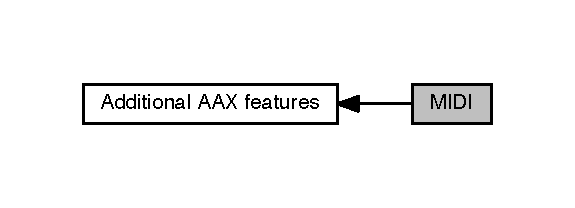
\includegraphics[width=276pt]{a00336}
\end{center}
\end{figure}
